
% this file is called up by thesis.tex
% content in this file will be fed into the main document

%: ----------------------- introduction file header -----------------------
\begin{savequote}[50mm]
Personally, I think it does help, that it makes a beneficial difference, but the scientific literature on the subject is very messy.
\qauthor{Jeanne Petrek}
%“And upon the top of the pillars was lily work: so was the work of the pillars finished.”
%
% Bible quotes
\end{savequote}


\chapter{Estado del Arte}
\label{cha:State of the Art}

% the code below specifies where the figures are stored
\ifpdf
    \graphicspath{{2_state_of_the_art/figures/PNG/}{2_state_of_the_art/figures/PDF/}{2_state_of_the_art/figures/}}
\else
    \graphicspath{{2_state_of_the_art/figures/EPS/}{2_state_of_the_art/figures/}}
\fi


%------------------------------------------------------------------------- 

Las competencias genéricas son las habilidades que los profesionales deben ser capaces de desempeñar independientemente de su especialización. Habilidades como el trabajo en equipo, la comunicación interpersonal, la capacidad para resolver problemas, la creatividad o el liderazgo, entre otras, son competencias que las empresas demandan hoy en día en los nuevos titulados, además de las competencias específicas que se les supone por la titulación que hayan terminado. Desde un punto de vista formativo, los profesores deben integrar estas competencias en sus asignaturas, tanto en las clases tradicionales como en los entornos virtuales. Y por supuesto, deben fijar mecanismos no sólo para el desarrollo de estas competencias, sino también para la evaluación de las mismas.

Los \emph{entornos virtuales de aprendizaje} (EVA o, del inglés, VLE, virtual learning environment) almacenan información de estudiantes, profesores, cursos, tareas, trabajos, etc. Estos elementos se relacionan y configuran para ofrecer al usuario una experiencia de curso virtual. Estos cursos están en auge hoy en día, siendo el soporte virtual de las clases presenciales o incluso siendo el único medio donde unas clases o un curso se imparten. Las clases virtuales presentan numerosas ventajas con respecto a las clases tradicionales. Por un lado se elimina la limitación geográfica que tienen las clases tradicionales, y por otro lado la oferta y variedad de cursos ofrecidos siempre será mayor. Además, para los estudiantes presentan otras ventajas fundamentales: en primer lugar la flexibilidad de horario, permitiéndoles compatibilizar los estudios con una vida laboral sin renunciar a crecer profesionalmente; y en segundo lugar, les permite estar en contacto permanente con otros estudiantes y profesores mediante diferentes herramientas (foros, chats, ... etc.)~\cite{alAjlan:2008}.

% VENTAJAS: http://oedb.org/ilibrarian/10-advantages-to-taking-online-classes/
Pero además de todo lo anterior, un EVA almacena una gran cantidad de información que adecuadamente analizada y presentada podría ser de gran utilidad para los profesores para monitorizar el trabajo de sus estudiantes~\cite{podgorelec:2011}. Cada archivo, cada acceso o cada tarea realizada por cada estudiante queda registrada en el sistema. Por desgracia, esta información no está siempre a disposición del profesor, y si lo está, requiere un filtrado para poder ser utilizada~\cite{Chebil:2012}. ¿Podrían utilizarse los registros de actividad de estos entornos para evaluar competencias genéricas?

En este capítulo se va a establecer la base teórica sobre la que se sustenta esta tesis doctoral. Se comenzará definiendo las preguntas de investigación, a las que se tratará de dar respuesta mediante un \emph{estudio de mapeo sistemático} (SMS, del inglés, Systematic Mapping Study). Un SMS, es una amplia revisión de los estudios primarios en un área específica cuyo objetivo es identificar alguna evidencia sobre el tema.

\section{Preguntas de investigación}

El objetivo principal de esta tesis doctoral es:

\bigskip
\textbf{\emph{Proponer un método para evaluar a los estudiantes en el desempeño de sus competencias genéricas mediante indicadores procedentes de los registros de actividades de aprendizaje.}}
\bigskip

Para abordar este objetivo ha de conocerse primero el estado del arte, dando respuesta para ello a diferentes preguntas de investigación. Las preguntas habrán de dar repuesta a interrogantes tales cómo cuáles son las competencias genéricas que se han evaluado haciendo uso de la informática, así cómo qué métodos se han utilizado y si se están usando para este fin los registros de actividad de los entornos virtuales.

\bigskip
Por tanto, partiendo del objetivo principal, se definen las siguientes preguntas de investigación:
\begin{itemize}
\item Q1. ¿Qué competencias se han evaluado de forma automática o asistida por ordenador a partir de la actividad de los estudiantes en los entornos virtuales?
\item Q2. ¿Qué métodos se utilizan para evaluar competencias genéricas mediante el uso de entornos virtuales?
\item Q3. ¿Qué técnicas se utilizan para evaluar competencias genéricas a partir de los registros de actividad de un entorno virtual?
\end{itemize}

\section{Metodología}

Un SMS es una amplia revisión de los estudios primarios en un área específica cuyo objetivo es identificar alguna evidencia sobre el tema. Este estudio se basa en las directrices publicadas en la metodología propuesta por Kitchenham \cite{Kitchenham:2010}. Esta metodología describe cómo se deben planificar, ejecutar y presentar los resultados de una revisión de la literatura en ingeniería del software. Para este trabajo se ha utilizado la propuesta de Petersen~\cite{Petersen:2008}.

\subsection{Protocolo de revisión}

La definición del protocolo de revisión requiere la realización de una serie de pasos para obtener la bibliografía de nuestro estudio. Los pasos a seguir son los siguientes:
\begin{enumerate}
\item Selección de motores de búsqueda (sección \ref{sec:MotoresBusqueda}).
\item Definición de los términos de búsqueda (sección \ref{sec:TerminosBusqueda}).
\item Determinación de los criterios de selección (sección \ref{sec:CriteriosBusqueda}).
\item Clasificación para la extracción de los datos (sección \ref{sec:EsquemaBusqueda}).
\end{enumerate}

%Comenzaremos indicando los motores de búsqueda que vamos a utilizar, qué términos de búsqueda utilizaremos en dichos motores y las herramientas de soporte a la revisión. Además se mostrarán qué criterios de inclusión de la bibliografía se siguen y el procedimiento de selección.

\subsection{Motores de búsqueda}
\label{sec:MotoresBusqueda}
Para encontrar la bibliografía, se realizarán consultas en las siguientes bibliotecas digitales: 
\begin{itemize}
\item Web of Science
\item Wiley Online Library
\item Science Direct
\item IEEE Digital Library (Xplore)
\end{itemize}

\subsection{Términos de búsqueda}
\label{sec:TerminosBusqueda}
Existen muchos términos que pueden utilizarse para referirse a la evaluación de competencias genéricas de manera automatizada o asistida. Por la naturaleza de nuestro trabajo, debemos contemplar siempre en las palabras de búsqueda los términos \emph{assessment} y \emph{generic skills} o \emph{generic competences}. Realizar la búsqueda por el término \emph{Assessment of generic skills} o \emph{assessing generic skills} devolvía muy pocos resultados. Por ejemplo, en la \emph{Wiley Online Library} la búsqueda del término exacto \emph{generic skills assessment} devolvió un único resultado. Sin embargo, debilitar la búsqueda con términos como \emph{generic competences} o \emph{generic skills} junto con la palabra \emph{assessment} daba un número de resultados muy elevado. En la misma biblioteca, buscar por los términos \emph{``generic skills`` and student and assessment} nos devolvía 609 resultados. En primera instancia se probó añadiendo términos como  \emph{E-Learning}, \emph{computer-assisted} o \emph{mobile learning}. Sin embargo, incluir términos de este tipo reducían también drásticamente el número de resultados obtenidos en la búsqueda, no llegando a obtenerse bibliografía más significativa que si no se incluyen. Por tanto, a tenor de las pruebas se decide eliminar de la búsqueda ese tipo de términos. La combinación de los términos de búsqueda empleados en la investigación, así como a los motores de búsqueda que fueron aplicados en cada una pueden comprobarse en la tabla \ref{tab:ResumenBusqueda}. Los términos de búsqueda se han empleado en todos los campos (título, resumen, texto, etc.).

%Por otro lado, sí se incluyen acrónimos de diferentes entornos virtuales relacionados con las TEL, como son: \emph{TEL}, \emph{LMS}, \emph{ICT} (Information and Communications Technology), \emph{CBI} (Content-Based Instruction). Y tras varias pruebas, se descartan también de la búsqueda términos como `\emph{ICE} (Integrated Collaboration Environment) y \emph{CSCL} (Computer Supported Collaborative Learning), debido a que son términos que en conjunción con los términos principales de nuestra búsqueda no suelen aparecer y los resultados de estas búsquedas eran nulos. Un ejemplo de esto se refleja en una de las consultas realizadas en \emph{Scopus}, dónde los términos \emph{((``student assessment`` OR ``assessment of students``) AND (``generic skills`` OR ``generic competences``)) AND CSCL} no devolvían ningún resultado. 

\begin{table}
  \begin{center}
  \begin{tabular}{| p{2.8cm} | p{5.5cm} | p{3cm} | p{0.8cm} |}
    \hline
    SOURCE & SEARCH TERMS & PUBLICATION & RSLT \\
    \hline
    \hline
    Web of Science & ((``generic competences`` OR ``generic skills``) AND assessment) & Journals & 138 \\
    \hline
    Wiley Online Library & ``generic competences`` AND assessment & Journals and Conferences & 50 \\
    \hline
    Science Direct & (``generic competences``) AND assessment) & Journals & 71 \\
    \hline
    IEEE Digital Library (Xplore) & ((``generic competences``) AND assessment) & Journals and Conferences & 54 \\
    \hline

%    Wiley Online Library & assessment AND ``generic competences`` OR ``generic skills`` AND (TEL OR ICT OR CBI) & in All Fields\\
%    World Scientific Net & ``generic competences`` OR ``generic skills`` AND assessment & Anywhere in article\\
%    Springer & (``generic skills`` OR ``generic competences``) AND  students AND (TEL OR CBI OR ICT) & All fields (Including full text)\\
%    ACM Digital Library & (assessment and ``generic skills``) and (TEL or LMS or ICT or CBI) & Any field (title, abstract, review)\\
%    ACM Digital Library & (assessment and ``generic competences``) and (TEL or LMS or ICT or CBI) & Any field (title, abstract, review)\\
%	  IEEE Digital Library (Xplore) & (((TEL or LMS or ICT or CBI) AND (``generic skills`` OR ``generic competences``)) AND assessment) & Full text and metadata\\
%    Scopus & (((TEL or LMS or ICT or CBI) AND (``generic skills`` OR ``generic competences``)) AND assessment) & All fields (Including full text)\\
    \hline
  \end{tabular}
\end{center}
\caption{Resumen de búsqueda de bibliografía}
\label{tab:ResumenBusqueda}
\end{table} 

\subsection{Criterios de selección}
\label{sec:CriteriosBusqueda}
Para determinar si un trabajo debía formar parte de nuestra selección de estudios primarios se leyó el título, el resumen y las palabras clave. Cuando esto no era suficiente se complementaba la lectura anterior con una somera la lectura del artículo completo, y más detallada de la introducción y las conclusiones.
Nuestra búsqueda se centró en la localización de los trabajos que, habiendo sido obtenidos en el proceso de búsqueda anterior, vayan en línea con nuestro estudio y puedan ayudarnos a resolver las preguntas de investigación. Para ello, se realizó la proyección de los trabajos seleccionados utilizando los siguientes criterios de exclusión:
\begin{itemize}
\item Included: trabajo relacionado con nuestra investigación.
\item Off Topic: trabajo no relacionado directamente con nuestra investigación. Son trabajos que satisfacen los criterios de búsqueda, pero cuya contribución no está directamente relacionada con la temática de este estudio. La mayoría de artículos descartados en este bloque consisten en experiencias que trabajan o mejoran alguna competencia genérica en los estudiantes, pero no mencionan si después el desempeño en la competencia se mide de alguna forma, y si por el contrario sí realizan una medición, lo hacen sin apoyo alguno de la tecnología.
\item Unsupported Language: trabajo escrito en un lenguaje diferente al inglés o español. La mayoría de los textos son en inglés, por lo que este criterio de descarte apenas es utilizado.
\item Duplicated: trabajos cuya contribución principal está recogida en otros trabajos ya incluidos. 
\item Unread: trabajo que no ha podido ser leído. Son textos que no han sido leídos al no estar disponible en las bibliotecas digitales a las que se tiene acceso desde la Universidad de Cádiz ni se ha podido encontrar por otros medios (petición por correo a los autores, búsqueda en otros repositorios de Internet, etc.).
\end{itemize}

\subsection{Esquema para la extracción de datos}
\label{sec:EsquemaBusqueda}

Para la extracción de la información se han dividido los trabajos de acuerdo a los siguientes tres aspectos: tipo de investigación, tipo de contribución y ámbito de aplicación de la investigación. A continuación se detalla esta clasificación.

\subsubsection{Tipo de investigación}
Esta clasificación hace referencia al tipo de trabajo de investigación llevado a cabo por el/los investigador/es. Existen diferentes enfoques para la clasificación de los trabajos según el tipo investigación que desarrollan. Algunos de estos sistemas de clasificación son los propuestos por Wieringa \cite{Wieringa:2005} y Hevner \cite{Hevner:2004}. Usamos el primero, ya que es el recomendado en el SMS descrito por Petersen \cite{Petersen:2008}.
\begin{itemize}
\item Solución propuesta (\emph{proposal of solution}): se propone una solución para un problema; la solución puede ser innovadora o una extensión significativa de una técnica existente. Los posibles beneficios y la aplicabilidad de la solución se demuestran por un pequeño ejemplo o una buena línea de argumentación.
\item Validación de investigación (\emph{validation research}): las técnicas investigadas son nuevas y todavía no se han aplicado en la práctica. Estas técnicas podrían ser por ejemplo los experimentos, es decir, el trabajo realizado en un laboratorio.
\item Evaluación de la Investigación (\emph{evaluation research}): las técnicas se aplican en la práctica y se lleva a cabo una evaluación de la técnica. Se muestra cómo se implementa la técnica en la práctica (implementación de la solución) y cuáles son las consecuencias de la aplicación en términos de ventajas y desventajas (evaluación de implementación).
\item Artículos de Experiencia (\emph{experience papers}): trabajos que explican qué y cómo algo se ha llevado a cabo en la práctica. Basado en la experiencia personal del autor.
\item Artículos de opinión (\emph{opinion papers}): estos trabajos expresan la opinión personal de alguien acerca de la bondad o viabilidad de una determinada técnica, o cómo se deben realizar las cosas. No se basan en metodologías de trabajo y de investigación relacionadas.
\item Trabajos filosóficos (\emph{philosophical papers}): estos trabajos esbozan una nueva forma de ver las cosas existentes, estructurando el campo en forma de una taxonomía o un marco conceptual.
\end{itemize}

\subsubsection{Tipo de contribución}
En este apartado se clasifican los trabajos según el tipo de contribución que realizan estos al ámbito en el que se desarrollan. Una vez realizado el estudio sistemático de la literatura y habiendo seleccionado los artículos, se realiza una clasificación en base a la aportación de éstos. El uso de algunos términos puede ser confuso, debido a la interpretación que hace el autor del mismo. Algunos de estos términos son framework, modelo, estrategia, proceso, procedimiento, método o metodología. Nuestra clasificación es la siguiente:
\begin{itemize}
\item Modelo (\emph{model}): es una representación de procesos, modelos o sistemas pertenecientes a un supra-sistema, cuyo fin es el análisis de interacción de ellos para mantener una relación flexible que les permita cumplir su función particular y cumplir la función de dicho supra-sistema.
\item Proceso (\emph{process}): contempla aquellos trabajos cuya contribución sea descrita por los autores como una serie de pasos.
\item Herramienta (\emph{tool}): se utiliza para los artículos que presentan un software independiente o una extensión de algún otro programa.
\item Framework (\emph{framework}): aquí se consideran aquellos trabajos que contribuyen con una combinación de los elementos anteriores (es decir, con un modelo, un proceso y una herramienta).
\item Técnica (\emph{technique}): un procedimiento utilizado para llevar a cabo una actividad o tarea específica. Podría venir acompañado de una herramienta de apoyo.
\end{itemize}

\subsubsection{Ámbito de aplicación de la investigación}
Además de las clasificaciones anteriores, es necesario recoger más información acerca los conceptos que representan la contribución de la investigación. Para ello se recoge información sobre el ámbito y la manera en que de la evaluación de competencias sobre el que se aplica cada contribución. Una vez recogida esta información, se agrupan según sus similitudes, quedando finalmente la siguiente clasificación:
\begin{itemize}
\item Evaluación del profesor (\emph{teacher assessment}): el profesor evalúa el desempeño de los estudiantes en una o varias competencias genéricas de manera asistida o semi-asistida por el ordenador.
\item Evaluación entre iguales y autoevaluación (\emph{peer and self-assessment}): uno de los problemas con los que se encuentran los profesores es la escalabilidad de la tarea de evaluación de competencias cuando el grupo de alumnos es grande. En estos trabajos, con el apoyo de la tecnología delegan parte o todo el proceso de evaluación en los estudiantes mediante la autoevaluación o evaluación entre iguales.
\item Cuestionarios (\emph{questionaries}): en este conjunto de trabajos que automatizan los procesos de evaluación mediante el uso de tests sicológicos orientados a alguna competencia en particular.
\item Herramientas de evaluación automática (\emph{automatic assessment tools}): en esta rama se recogen trabajos que automatizan el proceso de evaluación de competencias.
\end{itemize}

\subsection{Visualización y análisis de los datos}
Tras obtener los estudios primarios, hay una etapa de análisis, donde se resumen los datos extraídos para así responder a las preguntas de investigación planteadas. El análisis de los resultados se centra en el estudio de las publicaciones para cada categoría y por lo tanto, en la determinación del grado de cobertura de cada categoría. Esta información generalmente se resume en tablas y gráficos. Otro método utilizado en nuestro estudio es la combinación de diferentes categorías (por ejemplo, el ámbito de investigación contra el tipo contribución) y su representación en un mapa sistemático en la forma de un gráfico de burbujas.
En el siguiente capítulo se mostrarán los resultados obtenidos.

\section{Resultados}

A continuación se muestran los resultados del estudio. Comienza el capítulo con la localización de los estudios primarios, para continuar con la extracción de los datos de estudio, mostrándose varios gráficos y/o tablas que justifican la información mostrada. Finalmente se categorizan los estudios y se muestra el esquema de clasificación resultante.

\subsection{Localización de la literatura}

En la tabla \ref{tab:ResumenBusquedaResultados} se muestran las búsquedas realizadas en las bibliotecas digitales más importantes en ciencias de la computación, los términos de búsqueda utilizados y el número de documentos obtenidos. En cada biblioteca, se utilizaron los formularios de búsqueda avanzada y los resultados fueron obtenidos a fecha 21 de agosto de 2015. Toda la información de búsqueda de este SMS está disponible para su consulta \footnote{http://XXX.???}.

%\footnote{http://sms.antoniobalderas.es}.

\begin{table}
  \begin{center}
  \begin{tabular}{| p{4cm} | p{8cm} | r |}
    \hline
    SOURCE & SEARCH TERMS & RESULTS\\
    \hline
    \hline
    Web of Science & ((``generic competences`` OR ``generic skills``) AND assessment) & 50 \\
    \hline
    Wiley Online Library & ``generic competences`` AND assessment &  138 \\
    \hline
    Science Direct & (``generic competences``) AND assessment) &  71 \\
    \hline
    IEEE Digital Library (Xplore) & ((``generic competences``) AND assessment) & 54 \\
    \hline
    \hline
    \multicolumn{2}{|r|}{TOTAL} & 313\\
    \hline
  \end{tabular}
\end{center}
\caption{Bibliotecas digitales utilizadas, palabras de búsqueda utilizadas en cada uno y número de resultados obtenidos}
\label{tab:ResumenBusquedaResultados}
\end{table} 

En total se recopilaron 313 trabajos para ser revisados. El número de estudios primarios resultante (después de aplicar criterios de selección y exclusión) fue de 49 trabajos (casi un 16\% del total de trabajos recopilados). Aunque hay muchos trabajos que tratan las competencias genéricas desde diferentes perspectivas, son muy pocos los que abordan su evaluación con apoyo de tecnología. Los resultados de esta clasificación pueden verse en la tabla \ref{tab:ResumenSelecccionResultados}.

\begin{table}
  \begin{center}
  \begin{tabular}{| m{4cm} | r | r |}
    \hline
    CRITERIO & TRABAJOS & PORCENTAJE\\
    \hline
    \hline 
    Included & 49 & 15,65\% \\
    \hline
    Off Topic & 249 & 79,55\% \\
    \hline
    Unsupported Language & 0 & 0,00\% \\
    \hline
    Duplicated & 10 & 3,20\% \\
    \hline
    Unread & 5 & 1,60\% \\
    \hline
    TOTAL & 313 & 100,00\% \\
    \hline
  \end{tabular}
\end{center}
\caption{Clasificación de trabajos una vez aplicados los criterios de selección y exclusión}
\label{tab:ResumenSelecccionResultados}
\end{table} 

\subsection{Extracción de los datos}

Aunque las tecnologías entraron a formar parte de la vida académica hace ya varios años, no es hasta 2010, con la tercera generación de herramientas de medición educativa bajo el marco de la Comisión Europea (\emph{Generation 3: continuous integrated assessment}) \cite{Redecker:2013}, cuando se comienzan a integrar la evaluación en las herramientas de aprendizaje. Entonces conceptos como \emph{Data Mining and analysis}, \emph{Behavioural tracking} and \emph{Learning analytics} comienzan a usarse. Tanto en la tabla \ref{tab:ResumenAniosResultados} como en la figura \ref{fig:PublicacionesAnuales} puede verse la distribución de la producción de la selección primaria a lo largo de los años. Casi la mayor parte de los seleccionados se pueden localizar en los últimos años. Véase como 37 de estos trabajos (75,51\%) fueron publicado entre 2010 y 2015.

% Quitada coma tras véase (, véase) por mal uso. Estará mejor un punto y seguido?

\begin{table}
  \begin{center}
  \begin{tabular}{| m{4cm} | r | r |}
    \hline
    AÑOS & RESULTADOS & PORCENTAJE\\
    \hline    
    \hline
    2002 & 1 & 2,04\% \\
    \hline
    2003 & 0 & 0,00\% \\
    \hline
    2004 & 0 & 0,00\%\\
    \hline
    2005 & 1 & 4,08\%\\
    \hline
    2006 & 2 & 4,08\%\\
    \hline
    2007 & 3 & 6,12\%\\
    \hline
    2008 & 3 & 6,12\%\\
    \hline
    2009 & 2 & 4,08\%\\
    \hline
    2010 & 7 & 14,29\%\\
    \hline
    2011 & 10 & 20,41\%\\
    \hline
    2012 & 2 & 4,08\%\\
    \hline
    2013 & 9 & 18,37\% \\
    \hline
    2014 & 5 & 10,20\%\\
    \hline
    2015 & 4 & 8,16\% \\
    \hline
  \end{tabular}
\end{center}
\caption{Cantidad de trabajos publicados cada año}
\label{tab:ResumenAniosResultados}
\end{table}

\begin{figure}
  \begin{center}
    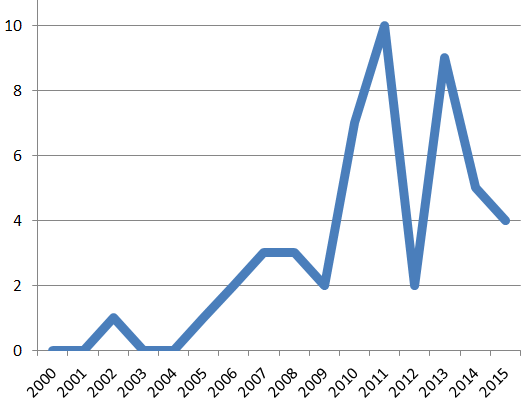
\includegraphics[scale=0.4]{PublicacionesAnuales.png}
  \end{center}
  \caption{Distribución de las publicaciones por años}
  \label{fig:PublicacionesAnuales}
\end{figure}

\subsection{Categorización del estudio}

Una vez revisados todos los artículos, se han extraído unas características o categorías comunes a la tipología de los trabajos. Todos los trabajos seleccionados hacen uso de algún tipo de software o metodología para evaluar una o varias competencias genéricas. En la tabla~\ref{tab:CompetenciasGenericas} se muestran las competencias genéricas que se evalúan en los trabajos seleccionados.


\pagestyle{empty}
\begin{landscape}
  \begin{center}
\begin{longtable}{| m{6cm} | m{16cm} |}
    \hline
    COMPETENCIA & DESCRIPCIÓN \\
    \hline
    \hline
    Análisis & Capacidad de abstracción, análisis y sintesis~\cite{gonzalez2003tuning}.\\
    \hline
    Aprendizaje permanente & Marco constituido por el aprendizaje formal, no formal e informal, que aspira a la adquisición de conocimiento para alcanzar el máximo desarrollo de la personalidad y de las destrezas profesionales en las diferentes etapas de la vida~\cite{bernheim2010educacion}. \\
    \hline
    Comunicación & Habilidad para comunicarse de manera tanto oral como escrita en la lengua materna~\cite{gonzalez2003tuning}. \\
    \hline
    Creatividad & Capacidad para crear nuevas ideas~\cite{gonzalez2003tuning}. \\
    \hline
    Cultural & Aprecio y respeto por la diversidad y la multiculturalidad~\cite{gonzalez2003tuning}. \\
    \hline
    Emprendimiento & Capacidad para tomar la iniciativa y espíritu de empresar~\cite{gonzalez2003tuning}. \\
    \hline
    Gestión de proyectos & Habilidades para diseñar y gestionar proyectos~\cite{gonzalez2003tuning}. \\
    \hline
    Habilidades interpersonales & Capacidad de la persona para comunicarse e interactuar con otras personas~\cite{gonzalez2003tuning}. \\ % De aqui: http://www.skillsyouneed.com/interpersonal-skills.html
    \hline    
    Investigación & Capacidad para llevar a cabo la investigación en un nivel apropiado~\cite{gonzalez2003tuning}.  \\
    \hline
    Liderazgo & Habilidad para motivar a la gente y conducirlos hacia un objetivo común~\cite{gonzalez2003tuning}. \\
    \hline
    Pensamiento crítico & Habilidad para interpretar, analizar y evaluar ideas y argumentos~\cite{fisher2011critical}. \\
    \hline
    Planificación y gestión del tiempo & Capacidad de planificar y gestionar el tiempo de manera efectiva~\cite{gonzalez2003tuning}. \\
    \hline
    Resolución de problemas & Habilidad para identificar, plantear y resolver problemas~\cite{gonzalez2003tuning}. \\
    \hline
    Responsabilidad & Capacidad para actuar con responsabilidad social y conciencia cívica~\cite{gonzalez2003tuning}. \\
    \hline 
    Segundo idioma & Capacidad de los estudiantes para comunicar sus ideas en un segundo idioma~\cite{gass2013second}. \\
    \hline
    TIC & Habilidades en el uso de las tecnologías de la información y de la comunicación~\cite{gonzalez2003tuning}. \\
    \hline
    Toma de decisiones & Capacidad para tomar deciciones razonadas~\cite{gonzalez2003tuning}. \\
    \hline
    Trabajo autónomo & Capacidad para trabajar de forma autónoma~\cite{gonzalez2003tuning}. \\
    \hline
    Trabajo en equipo & Trabajo realizado por un conjunto de personas en aras de un objetivo común~\cite{parker1990teamwork}. \\
    \hline
\caption{Competencias genéricas}
\label{tab:CompetenciasGenericas}
\end{longtable} 
\end{center}
\end{landscape}
\pagestyle{fancy}

De los trabajos seleccionados, sólo dos mencionan un enfoque como el que se propone en la introducción de este capítulo, es decir, aprovechando los registros de interacción de los estudiantes con el LMS como indicadores del desempeño de las competencias genéricas. Encontramos trabajos que se apoyan en la tecnología para el tratamiento o evaluación de las competencias, pero que terminan delegando parte de esta evaluación en el alumnado, ya sea mediante autoevaluación o evaluación entre iguales. Otros trabajos se basan en videojuegos o en las redes sociales para evaluar alguna competencia, mientras que otros desarrollan algún tipo de software o técnica. Finalmente hay algunos trabajos que simplemente detectan en su entorno la necesidad de la evaluación de las competencias de manera automática porque su forma de hacerlo les ocasiona una serie de problemas o desventajas con respecto a otro método que proponen o demandan. Algunos trabajos utilizan más de un método simultáneamente. En la tabla \ref{tab:PublicacionesForum} se puede ver la distribución de las publicaciones. Además, nos encontramos con una revisión de la literatura sobre las competencias genéricas más evaluadas. Dicha revisión se utilizará para contrastar los datos sobre esas competencias con los obtenidos en este mapeado para responder a la primera pregunta de investigación. %, apoyadas gráficamente en la figura  \ref{fig:PublicacionesForum}.

\begin{table}
  \begin{center}
  \begin{tabular}{| m{10cm} | c |}
    \hline
    CATEGORÍA & TRABAJOS\\
    \hline
    \hline 
    Evaluación entre iguales y autoevaluación & 21\\
    \hline
    Evaluación del profesor & 22\\
    \hline
    Cuestionarios & 14\\
    \hline
    Herramientas de evaluación automática & 4\\
    \hline
  \end{tabular}
\end{center}
\caption{Distribución de publicaciones por tratamiento del problema}
\label{tab:PublicacionesForum}
\end{table} 

%\begin{figure}
%  \begin{center}
%    \includegraphics[scale=0.4]{cap3_pub_forum.png}
%  \end{center}
%  \caption{Distribución de publicaciones por tratamiento del problema}
%  \label{fig:PublicacionesForum}
%\end{figure}

En la figura \ref{fig:Burble} se muestra la clasificación de los trabajos según su ámbito y su tipo (lado izquierdo), y según su ámbito y su contribución (lado derecho). La mayoría de los trabajos son propuestas (\emph{Proposal of solution}), experiencias (\emph{Experience papers}), validaciones (\emph{Validation research}) y evaluaciones de la investigación (\emph{Evaluation research}), mientras que trabajos trabajos típicos de un tema de investigación de cierta madurez como los de opinión (\emph{Opinion papers}) y los filosóficos (\emph{Philosophical papers}) casi no hay. %Ésto junto con el hecho de haber hallado pocos trabajos confirma el poco tratamiento de este tema en la investigación. 

El tipo de contribución está más distribuido. Las contribuciones del tipo proceso (\emph{Process}) y modelo (\emph{Model}) son las que se dan con más frecuencia: la primera con cuestionarios (\emph{Questionnarie}), evaluación del profesor (\emph{Teacher assessment}) y autoevaluaciones o evaluaciones entre compañeros (\emph{Peer and self-assessment}), mientras que la segunda se da con más frecuencia con cuestionarios y evaluaciones del profesor. 

\pagestyle{empty}
\begin{landscape}
\begin{figure}[H]
  \begin{center}
    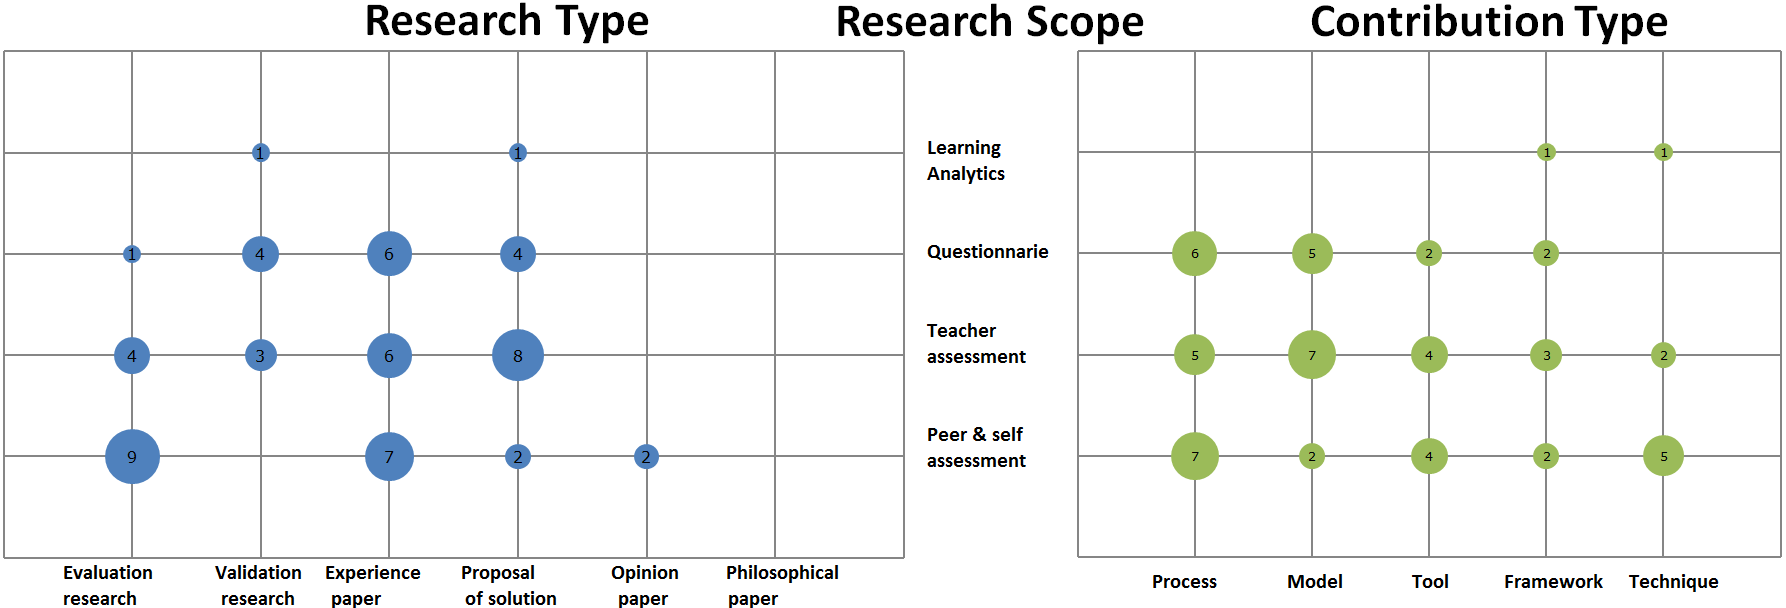
\includegraphics[scale=0.4]{Burbujas.png}
  \end{center}
  \caption{Ámbito de trabajos distribuidos según tipo de investigación y según tipo de contribución.}
  \label{fig:Burble}
\end{figure}
\end{landscape}
\pagestyle{fancy}

% Original pre-revision Juanma: EsquemaClasificacion.tex

\subsection{Esquema de clasificación}

En los apartados siguientes, se presentan los resultados del estudio para cada área de investigación. El listado de trabajos se muestra en la tabla~\ref{tab:ListadoTrabajos}.

\subsubsection{Evaluación entre iguales y autoevaluación (peer and self-assessment)}

La autoevaluación es un proceso en el que los estudiantes evalúan su propio trabajo, mientras que  en el proceso de evaluación entre iguales un estudiante evalúa el trabajo de otro u otros estudiantes. Esta práctica se emplea por un lado para ahorrar tiempo del profesorado, y por otro, para mejorar tanto el conocimiento en la materia del alumnado como sus habilidades metacognitivas. A menudo este tipo de evaluación se acompaña de algún tipo de rúbrica \cite{malehorn1994ten}.

Se han encontrado muchos trabajos en la literatura que utilizan este enfoque para evaluar competencias genéricas. De acuerdo a las preguntas de investigación de este trabajo únicamente se han recopilado aquellos trabajos que bajo este enfoque hagan uso de los ordenadores.

\bigskip
\textbf{Competencias evaluadas}
\bigskip

El \emph{trabajo en equipo} es la competencia más evaluada mediante este proceso de evaluación, ya que encontramos varios trabajos en los que después de realizar un trabajo en equipo los estudiante se evalúan unos a otros (evaluación entre iguales)~\cite{ficapal2015learning,barbera2011assessment,khamis2012measurement}. También adquieren protagonismo competencias relacionadas con el trabajo en equipos, como son la \emph{comunicación} y la \emph{responsabilidad}. El espíritu empresarial (\emph{emprendimiento}) y el \emph{idioma} son las otras competencias que destacan dentro de este grupo de procesos de evaluación. En la tabla~\ref{tab:CompetenciasAuto} se puede ver el listado de trabajos para cada competencia.

% starcic2008sustaining: Pregunta a profesores por todas las competencias mediante cuestionario sobre lo bueno de utilizar e-portfolio
% so2011mapping: solo se ha leído el abstract y no se especifican

\begin{table}
  \begin{center}
  \begin{tabular}{| m{3.5cm} | m{9cm} |}
    \hline
    COMPETENCIA & TRABAJOS\\
    \hline
    \hline
    Análisis & \cite{sin2007evaluating,carreras2013promotion,lasa2013problem} \\
    \hline
    Comunicación &  \cite{masip2013self,barbera2011assessment,ruizacarate2013soft,sin2007evaluating,carreras2013promotion,johnson2002encouraging} \\
    \hline
    Creatividad & \cite{piedra2010measuring} \\
    \hline
    Emprendimiento & \cite{DeXena2012educacion,chang2009international,marquez2010have,achcaoucaou2014competence} \\
    \hline
    Pensamiento crítico & \cite{arno2011promoting,pinto2011assessment} \\
    \hline
    Responsabilidad & \cite{ruizacarate2013soft,carreras2013promotion} \\
    \hline
    Resolución de problemas & \cite{johnson2002encouraging} \\
    \hline 
    Segundo idioma & \cite{renau2010teaching,masip2013self,sevilla2012assessment} \\
    \hline
    TIC & \cite{lasa2013problem} \\
    \hline
    Trabajo autónomo &  \cite{lasa2013problem} \\
    \hline
    Trabajo en equipo &  \cite{masip2013self,ficapal2015learning,khamis2012measurement,barbera2011assessment,ruizacarate2013soft,piedra2010measuring,mcloughlin2006beyond,carreras2013promotion,lasa2013problem,johnson2002encouraging} \\
    \hline
  \end{tabular}
\end{center}
\caption{Competencias evaluadas mediante autoevaluación y evaluación entre iguales}
\label{tab:CompetenciasAuto}
\end{table} 

\bigskip
\textbf{Estrategias}
\bigskip

Los trabajos seleccionados en esta parte siguen todos una estrategia muy parecida. Se utilizan una o varias herramientas y después se realizan cuestionarios de autoevaluación o evaluación entre compañeros. También podemos encontrar algún trabajo en el que el cuestionario también se pasa antes de aplicar la herramienta. A continuación se describen las diferentes estrategias encontradas, con los elementos que en ella aparecen y en la tabla~\ref{tab:MetodosAuto} se muestran los trabajos asociados a cada una:

\begin{itemize}
\item \emph{Metodología ABP}: trabajos que implementan una metodología de \emph{aprendizaje basado en problemas} (ABP o, del inglés, PBL, problem-based learning) para desarrollar competencias específicas y genéricas en sus estudiantes y que después se evalúan mediante rúbricas de autoevaluación y evaluación entre iguales.
\item \emph{Practicas con herramientas empresariales}: herramientas ligadas al ámbito empresarial (contabilidad, gestión de equipos, gestión de proyectos, ... etc.) acompañadas de rúbricas de autoevaluación.
\item \emph{Trabajo en E-Portfolio}: un e-portfolio (del inglés \emph{electronic portfolio}), consiste en un conjunto de documentos, generalmente textos, archivos e imágenes, gestionados en un entorno web por un usuario. Se han recopilado trabajos donde los estudiantes trabajan con esta herramienta durante el curso y al final autoevalúan el desempeño de alguna competencia genérica
\item \emph{Cuestionarios de nivel}: cuestionarios que miden el nivel de los estudiantes en el desempeño competencias genéricas previamente al inicio de una actividad o un curso.
\item \emph{Trabajo en equipo en plataforma online}: tras haber trabajado los estudiantes en equipos en un entorno de aprendizaje virtual se realizan cuestionarios de autoevaluación y evaluación entre iguales para medir su desempeño en diferentes competencias genéricas.
\end{itemize}


\begin{table}
  \begin{center}
  \begin{tabular}{| m{3.5cm} | m{3.5cm} | m{5.5cm} |}
    \hline
    MÉTODO & EVALUACIÓN & TRABAJOS\\
    \hline
    \hline
    Metodología ABP & Autoevaluación y evaluación entre iguales &  \cite{lasa2013problem,renau2010teaching,johnson2002encouraging,masip2013self} \\
    \hline
    Practicas con herramientas empresariales & Autoevaluación &  \cite{chang2009international,achcaoucaou2014competence} \\
    \hline
    Trabajo en E-Portfolio & Autoevaluación &  \cite{arno2011promoting,starcic2008sustaining} \\
    \hline
    Cuestionarios de nivel & Autoevaluación &  \cite{sevilla2012assessment,so2011mapping} \\
    \hline
    Trabajo en equipo en plataforma online & Autoevaluación y evaluación entre iguales &  \cite{ficapal2015learning,khamis2012measurement,barbera2011assessment,ruizacarate2013soft,piedra2010measuring,pinto2011assessment,carreras2013promotion} \\
    \hline
  \end{tabular}
\end{center}
\caption{Métodos utilizados en la autoevaluación y evaluación entre iguales}
\label{tab:MetodosAuto}
\end{table} 

% En \cite{mcloughlin2006beyond} se presentan una revisión de herramientas online para trabajar y evaluar competencias genéricas. Entre ellas también se mencionan herramientas colaborativas para la competencia del \emph{trabajo en equipo}. 


%Cuestionario			\cite{marquez2010have}		Sólo resumen y no veo referencia tecnológica: Lo quitaría auqnue habría que quitarlo de todos los informes, estadísticas, ... etc.

% Quitar también sin2007evaluating

\bigskip
\textbf{Limitaciones}
\bigskip

Aunque la autoevaluación y evaluación entre iguales son enfoques que quitan trabajo al docente, no todos son ventajas. En algunos trabajos anteriores, este enfoque a menudo sólo se utiliza de manera complementaria a algún otro tipo de evaluación~\cite{lasa2013problem,sevilla2012assessment,khamis2012measurement,barbera2011assessment,pinto2011assessment}. Además, se puede dar el caso que la autoevaluación no se ajuste del todo a la realidad del desempeño del estudiante. Por ejemplo, en~\cite{carreras2013promotion} hay notables diferencias entre las calificaciones que se auto-asignan los estudiantes en algunas competencias y las calificaciones que le asignaron los profesores en esas mismas competencias. En ese trabajo se promovió la adquisición de competencias genéricas desde un punto de vista interdisciplinar y se diseñaron herramientas específicas para evaluar dichas habilidades. A la hora de evaluar, se realizaron tanto autoevaluaciones como evaluaciones del profesor. En esta experiencia se evaluaron cuatro competencias genéricas: \emph{capacidad de análisis},  \emph{habilidades de escritura}, \emph{responsabilidad} y \emph{capacidad de trabajo en equipo}. Cabe destacar discrepancias entre las calificaciones que se auto-asignan los estudiantes en las dos primeras competencias. En la \emph{capacidad de análisis} la discrepancia es de un 55,65\%, mientras que en las \emph{habilidades de escritura} de un 13,75\%.

\subsubsection{Evaluación del profesor (teacher assessment)}

En muchos casos la evaluación de competencias genéricas se realiza mediante un seguimiento continuo del trabajo del estudiante por parte del profesor. Este proceso es lo que se conoce como \emph{evaluación continua}. Esto permite ir introduciendo mejoras constantes en el proceso de aprendizaje, siendo éste el motivo por el que la evaluación continua se adopta como una estrategia de evaluación formativa más orientada al proceso de aprendizaje que a una valoración puntual. Actualmente, los expertos, influenciados por la \emph{Declaración de Bolonia}, consideran más apropiado desarrollar este tipo de sistemas de evaluación~\cite{garcia2005competencias}. 

% Todas competencias en \cite{serrano2013hiperion}, se queda fuera de la tabla porque no habla de ninguna en concreto, sino de trabajo futuro.


\bigskip
\textbf{Competencias evaluadas}
\bigskip

Las competencias genéricas más evaluadas por este método son las de \emph{comunicación} y la de \emph{trabajo en equipo}. En la tabla~\ref{tab:CompetenciasProfesor} puede ver la relación de competencias evaluadas y los trabajos.

\begin{table}
  \begin{center}
  \begin{tabular}{| m{3.5cm} | m{9cm} |}
    \hline
    COMPETENCIA & TRABAJOS\\
    \hline
    \hline
    Comunicación & \cite{martin2010new,prashar2010competence,martin2013acquired,rodriguez2010portfolio,benlloch2007adapting,yang2014fine,lacuesta2009active,casan2015developing} \\
	\hline
	Emprendimiento & \cite{ward2011developing} \\
	\hline
	Pensamiento crítico & \cite{lacuesta2009active} \\
	\hline
	Planificación y gestión del tiempo & \cite{lacuesta2009active} \\
	\hline
	Resolución de problemas & \cite{martin2013acquired,rodriguez2010portfolio,benlloch2007adapting} \\    
    \hline
    Trabajo en equipo & \cite{martin2010new,prashar2010competence,martin2013acquired,rodriguez2010portfolio,benlloch2007adapting,lacuesta2009active} \\    
    \hline
  \end{tabular}
\end{center}
\caption{Competencias evaluadas por el profesor}
\label{tab:CompetenciasProfesor}
\end{table} 


\bigskip
\textbf{Estrategias}
\bigskip

En este trabajo nos encontramos con dos estrategias básicas: por un lado estrategias basadas en la evaluación continua, en la que los profesores recogen evidencias del trabajo de los estudiantes en entornos virtuales durante el curso con las que rellenan rúbricas, hojas de cálculo o la herramienta de evaluación que utilicen. Por otro lado, tenemos estrategias basadas en evaluaciones finales, donde los profesores lo que evaluan es un resultado final del trabajo del alumno. En la tabla~\ref{tab:MetodosProfesor} puede ver los métodos que sigue cada uno de los trabajos que se han recopilado para este tipo de evaluación.

\begin{table}
  \begin{center}
  \begin{tabular}{| m{3.5cm} | m{3.5cm} | m{5.5cm} |}
    \hline
    MÉTODO & EVALUACIÓN & TRABAJOS\\
    \hline
    \hline
    Metodología ABP & Profesor &  \cite{lacuesta2009active} \\
    \hline
    Indicadores para evaluación continua & Profesor &  \cite{martin2010new,prashar2010competence} \\
    \hline
    Trabajo en e-portfolio & Estudiantes y Profesor &  \cite{martin2013acquired,rodriguez2010portfolio,benlloch2007adapting} \\
    \hline
    Modelo matemático evaluado por etapas & Profesor &  \cite{yang2014fine} \\
    \hline
    Módulos Moodle competencias empresariales & Profesor &  \cite{ward2011developing} \\
    \hline
    Rúbricas & Profesor &  \cite{casan2015developing} \\
    \hline
  \end{tabular}
\end{center}
\caption{Métodos utilizados en la evaluación de los profesores}
\label{tab:MetodosProfesor}
\end{table}


\bigskip
\textbf{Limitaciones}
\bigskip

Uno de los problemas de la no automatización de los procesos de evaluación es la escalabilidad de algunos procesos de evaluación. En~\cite{serrano2013hiperion} se diseña \emph{Hiperion}, una sistema de recomendación que ayuda a diseñar actividades adaptadas a cada estudiante para mejorar sus competencias. En el estudio de caso mostrado en este trabajo, los profesores evaluaban las competencias de los estudiantes manualmente y después aplicaban Hiperion. La principal desventaja de la herramienta es el tiempo que el profesor ha de dedicar para asignar los diferentes logros y el peso de cada nota para cada competencia en las actividades.

Siguiendo con los problemas de escalabilidad nos encontramos con el trabajo mostrado en~\cite{lacuesta2009active}. En él se utiliza una metodología ABP, en la que se realiza una evaluación individualizada de cada estudiante y de cada grupo de estudiantes. El autor considera también que el esfuerzo necesario y carga de trabajo para cada profesor es un poco mayor al habitual. 

\subsubsection{Cuestionarios (Questionnaries)}

Algunos de los cuestionarios que se han encontrado dentro de la bibliografía son tests de personalidad. Este tipo de cuestionario está diseñado para revelar aspectos del carácter o mecanismos psicológicos de un individuo. La evaluación de la personalidad se puede ver como la aplicación de procedimientos para medir aspectos de la personalidad de manera que sean aplicables a otros dominios~\cite{wiggins2003paradigms}. 

\bigskip
\textbf{Competencias evaluadas}
\bigskip

Uno de esos dominios es el laboral, sobre todo las entrevistas de trabajo. Es común la necesidad del empresario por conocer la aptitud o no del candidato a un puesto para asumir cierto rol dentro de una empresa. Todas las competencias están relacionadas por tanto con características de los encuestados que sean de interés para los empleadores (trabajo en equipo, responsabilidad, comunicación, habilidades interpersonales, cratividad, gestión de proyectos, liderazgo, resolución de problemas, etc.). En la tabla~\ref{tab:CompetenciasCuestionarios} se muestran las competencias evaluadas y los trabajos en que se evalúan.

\begin{table}
  \begin{center}
  \begin{tabular}{| m{3.5cm} | m{9cm} |}
    \hline
    COMPETENCIA & TRABAJOS\\
    \hline
    \hline
    Análisis & \cite{lumsden2005assessment} \\	  
    \hline
    Comunicación & \cite{martinez2014teamwork,barbera2011design,badcock2010developing} \\	  
    \hline
    Creatividad & \cite{albergaria2011critical} \\	  
    \hline
    Gestión de proyectos & \cite{martinez2014teamwork,barbera2011design} \\	  
    \hline
    Habilidades interpersonales & \cite{martinez2014teamwork,badcock2010developing} \\	  
    \hline
    Idioma & \cite{fernandez2011experience} \\  
    \hline
    Liderazgo & \cite{martinez2014teamwork} \\	  
    \hline
    Pensamiento crítico & \cite{badcock2010developing,albergaria2011critical} \\	  
    \hline
    Planificación y gestión del tiempo & \cite{martinez2014teamwork} \\	  
    \hline
    Resolución de problemas & \cite{badcock2010developing,vizcarro2013assessment} \\	  
    \hline
    Responsabilidad & \cite{lumsden2005assessment,park2006moral} \\	  
    \hline
    Trabajo en equipo & \cite{martinez2014teamwork,barbera2011design} \\	  
    \hline
  \end{tabular}
\end{center}
\caption{Competencias evaluadas mediante cuestionarios}
\label{tab:CompetenciasCuestionarios}
\end{table} 

\bigskip
\textbf{Estrategias}
\bigskip

En esta sección se muestran diferentes herramientas que consisten en cuestionarios para la evaluación automática de competencias genéricas (tabla~\ref{tab:MetodosCuestionarios}).

\begin{table}
  \begin{center}
  \begin{tabular}{| m{3.5cm} | m{3.5cm} | m{5.5cm} |}
    \hline
    MÉTODO & EVALUACIÓN & TRABAJOS\\
    \hline
    \hline
    ABP & Test &  \cite{barbera2011design} \\
    \hline
    Cuestionario preguntas abiertas & Test &  \cite{albergaria2011critical,vizcarro2013assessment} \\
    \hline
    GSA (Graduate Skills Assessment) & Test &  \cite{badcock2010developing} \\
    \hline
    Herramienta PQA (Personal Quality Assessment) & Test &  \cite{lumsden2005assessment} \\
    \hline
    TWBQ (Team Work Behaviour Questionnaire) & Cuestionario &  \cite{park2006moral} \\
    \hline
    VIA-Youth (Values in Action Invetory for Youth) & Cuestionario &  \cite{park2006moral} \\
    \hline
  \end{tabular}
\end{center}
\caption{Tipos de cuestionarios}
\label{tab:MetodosCuestionarios}
\end{table}

Simple test idioma: \cite{fernandez2011experience}
Modelos matemáticos \emph{Rasch model} y \emph{ESPEGS model}: su entrada es las evaluaciones tomadas por el profesor: \cite{aziz2007appraisal,rashid2008engineering,a2007outcome}

\bigskip
\textbf{Limitaciones}
\bigskip

El diseño de cuestionarios que reflejen aspectos de la personalidad es un trabajo de expertos. En \cite{andre2011formal} se propuso un modelo formal para asignar trabajadores a proyectos software. Para definir el modelo se siguió un método Delphi, donde un grupo de expertos definieron criterios para la evaluación de habilidades de trabajo en equipo y definieron un test psicológico. La creación de estos test psicológicos no está al alcance de todos los profesores.

Volvemos a encontrarnos con problemas de escalabilidad. El profesorado que participó en la experiencia de \cite{barbera2011design} reconoció que tuvieron que dedicar un elevado número de horas, tanto para las clases como para la evaluación de muchos proyectos. Más aun si los cuestionarios constan de preguntas abiertas y cerradas. Las preguntas abiertas obligan al evaluado a formular la respuesta a la pregunta y al evaluador a leerla para corregirla, lo que conlleva una mayor carga de trabajo. En \cite{albergaria2011critical} se presenta un cuestionario para evaluar el \emph{pensamiento crítico}, la \emph{curiosidad} y la \emph{creatividad}. El cuestionario consta sobre todo de preguntas abiertas, lo que implica tener que dedicar más tiempo y recursos para realizar las evaluaciones. En~\cite{vizcarro2013assessment}, profesores de los grados de Computación y Matemáticas y de Ingeniería Informática elaboraron una prueba escrita para la evaluación de la competencia genérica de \emph{resolución de problemas}. Este constaba de preguntas abiertas y cerradas, siendo minuciosamente seleccionadas por el profesorado que formaba parte en la experiencia, así como las respuestas que se esperarían de los estudiantes. El proyecto fue muy satisfactorio, aunque en las conclusiones vemos que los autores indican que encontrar un equilibrio entre el esfuerzo necesario para desarrollar este tipo de dispositivos de evaluación y la posibilidad de no hacerlo, o hacerlo pero no tan exhaustivamente, es algo que la comunidad académica debe abordar seriamente.



% JUEGOS SERIOS BASADOS EN INDICADORES: ¿LOS SACO DE LA?

\subsubsection{Herramientas de evaluación automática (automated assessment tools)}

Los juegos serios (\emph{serious game}) son juegos diseñados para un propósito principal distinto del de la pura diversión~\cite{djaouti2011classifying}. Normalmente, el adjetivo "serio" pretende referirse a productos utilizados por industrias como la de defensa, educación, exploración científica, sanitaria, urgencias, planificación cívica, ingeniería, religión y política~\footnote{http://cs.gmu.edu/~gaia/SeriousGames/index.html}. Los serios juegos son muy utilizados hoy en día en el aula, aunque son más aplicados a competencias específicas que a genéricas. En \cite{guenaga2013serious} se utilizan los juegos serios para el desarrollo de las competencias de \emph{emprendimiento} y \emph{solución de problemas}. Se definieron una serie de indicadores como medida del desempeño en las competencias que permiten al estudiante conocer su nivel de adquisición de las mismas. En \cite{bedek2011behavioral} también se utilizan los juegos serios para el desarrollo y evaluación de competencias genéricas. Se basa en un modelo donde para cada competencia se identifican subcompetencias más específicas, lo que facilita el proceso de definición de indicadores.

El término \emph{Learning Analytics}, traducido al español como análisis del aprendizaje, es definido por la \emph{Society for Learning Analytics} como la medición, recopilación, análisis y presentación de datos sobre los estudiantes, sus contextos y las interacciones que allí se generan, con el fin de comprender el proceso de aprendizaje que se está desarrollando y optimizar los entornos en los que se produce~\cite{siemens2012learning}.

En \cite{fidalgo:2015} también abordan la evaluación de la competencia de \emph{trabajo en equipo}. Pero en este caso se hace desde un enfoque completamente diferente. En este trabajo se propone utilizar indicadores basados en la interacción entre los agentes que intervienen en el proceso de aprendizaje: Mediante los mensajes escritos en el foro se mide la interacción estudiante-estudiante activo, mientras que mediante las lecturas en el foro se mide las interacciones estudiante-estudiante pasivo. En este trabajo los autores demuestran cómo estos indicadores están relacionados con el rendimiento trabajando en equipo de los estudiante. Además, cómo la obtención de estos indicadores mediante los mecanismos de un entorno virtual es un trabajo tedioso y lento, se desarrolló en este mismo trabajo el software \emph{LA system (Learning Analytics system)}.

En~\cite{rayon2014web} se propone la evaluación de varias competencias genéricas mediante indicadores obtenidos del análisis del proceso de aprendizaje (learning analytics). Para ello se crea una plataforma web llamada LACAMOLC (\emph{Learning Analytics for Competence Assessment of MObile Learning Contexts}), un panel que da soporte a los procesos de aprendizaje y evaluación proporcionando una perspectiva visual del análisis del aprendizaje mediante la recolección de datos sociales y de uso desde diferentes entornos de aprendizaje como Moodle, Google Apps para la educación y MediaWiki. Mediante LACAMOLC el profesor centraliza todos los indicadores para la evaluación de competencias obteniendo una información cuantitativa y visual. Mediante el número de accesos al foro de Moodle o mediante el número de contribuciones en el foro, se evalúan competencias como la \emph{comunicación interpersonal} o las \emph{habilidades de escritura}. También se utilizan indicadores obtenidos de documentos Google (\emph{Google Docs}).

\pagestyle{empty}
\begin{landscape}
\begin{center}
\begin{longtable}{| m{2.5cm} | m{9cm} | m{4cm} | m{2.5cm} | m{3.5cm} |}
    \hline
    REF & TÍTULO & TIPO DE INVESTIGACIÓN & TIPO DE CONTRIBUCIÓN & ÁMBITO DE LA INVESTIGACIÓN \\
    \hline
    \hline 
    \cite{yang2014fine} & A Fine-Grained Outcome-Based Learning Path Model & proposal of solution & model & Teacher assessment \\
    \hline
    \cite{rayon2014web} & A web platform for the assessment of competences in Mobile Learning Contexts & validation research & framework & Learning analytics \\
    \hline
    \cite{martin2013acquired} & Acquired Skills With The Implementation Of New Evaluation Methods At University Rey Juan Carlos & experience paper & model & Teacher assessment \\
    \hline
    \cite{lacuesta2009active} & Active learning through problem based learning methodology in engineering education & experience paper & process & Teacher assessment \\
    \hline
    \cite{benlloch2007adapting} & Adapting teaching and assessment strategies to enhance competence-based learning in the framework of the european convergence process & proposal of solution & process & Teacher assessment / Questionnarie \\
    \hline
    \cite{aziz2007appraisal} & Appraisal of Course Learning Outcomes using Rasch Measurement: A Case Study in Information Technology Education & proposal of solution & model & Questionnarie / Teacher assessment \\
    \hline
    \cite{sevilla2012assessment} & Assessment of competences in designing online preparatory materials for the Cambridge First Certificate in English examination & evaluation research & technique & Peer and self-assessment / Teacher assessment \\
    \hline
    \cite{lumsden2005assessment} & Assessment of personal qualities in relation to admission to medical school & evaluation research & framework & Questionnarie \\
    \hline
    \cite{vizcarro2013assessment} & Assessment of problem solving in computing studies & experience paper & process & Questionnarie \\
    \hline
    \cite{pinto2011assessment} & Assessment Of Self-Criticism Capacity Competence In Higher Education Students: Outcome Oriented Education & experience paper & process & Peer and self-assessment \\
    \hline
    \cite{barbera2011assessment} & Assessment Tools For The Evaluation Of Generic Skills Development In Students Of Business Management & proposal of solution & model & Teacher assessment \\
    \hline
    \cite{mcloughlin2006beyond} & Beyond marks and measurement: Developing dynamic and authentic forms of e-assessment & opinion paper & technique & Peer and self-assessment \\
    \hline
    \cite{achcaoucaou2014competence} & Competence Assessment in Higher Education: A Dynamic Approach & proposal of solution & tool & Peer and self-assessment \\
    \hline
    \cite{prashar2010competence} & Competence Based Teaching And Evaluation In The General Chemistry Course Of The University Rey Juan Carlos & experience paper & framework & Teacher assessment \\
    \hline
    \cite{strijbos2015criteria} & Criteria and standards of generic competences at bachelor degree level: A review study & evaluation research & process & Review study \\
    \hline
    \cite{albergaria2011critical} & Critical Thinking, Questioning and Creativity as Components of Intelligence & proposal of solution & process & Questionnarie \\
    \hline
    \cite{barbera2011design} & "Design And Results Of Collaborative Project-Based Learning In The Subject Commercial Management"" In Industrial Organization Engineering""" & experience paper & framework & Questionnarie \\
    \hline
    \cite{ward2011developing} & Developing entrepreneurial accounting and finance competency using the ELLEIEC Virtual Centre for Enterprise & experience paper & tool & Teacher assessment \\
    \hline
    \cite{badcock2010developing} & Developing generic skills through university study: a study of arts, science and engineering in Australia & experience paper & model & Questionnarie \\
    \hline
    \cite{casan2015developing} & Developing Writing Skills in The Classroom: A Corpus-based Analysis of Multi-Genre Structures & proposal of solution & model & Teacher assessment \\
    \hline
    \cite{ficapal2015learning} & e-Learning and Team-based Learning. Practical Experience in Virtual Teams & experience paper & framework & Peer and self-assessment / Questionnarie \\
    \hline
    \cite{johnson2002encouraging} & Encouraging generic skills in science courses & proposal of solution & process & Peer and self-assessment / Teacher assessment \\
    \hline
    \cite{rashid2008engineering} & Engineering Students Performance Evaluation of Generic Skills Measurement: ESPEGS Model & validation research & model & Questionnarie / Teacher assessment \\
    \hline
    \cite{rodriguez2010portfolio} & e-Portfolio: A tool to assess university students' skills & evaluation research & tool & Teacher assessment \\
    \hline
    \cite{sin2007evaluating} & Evaluating a method of integrating generic skills with accounting content based on a functional theory of meaning & evaluation research & process & Peer and self-assessment / Teacher assessment \\
    \hline
    \cite{andre2011formal} & Formal model for assigning human resources to teams in software projects & validation research & model & Questionnarie \\
    \hline
    \cite{bedek2011behavioral} & From Behavioral Indicators to Contextualized Competence Assessment & proposal of solution & framework & Teacher assessment \\
    \hline
    \cite{oliver2013graduate} & Graduate attributes as a focus for institution-wide curriculum renewal: innovations and challenges & opinion paper & model & Peer and self-assessment \\
    \hline
    \cite{marquez2010have} & Have Our Future Entrepreneurs An Ethical Commitment? & evaluation research & process & Peer and self-assessment \\
    \hline
    \cite{serrano2013hiperion} & Hiperion: A fuzzy approach for recommending educational activities based on the acquisition of competences & proposal of solution & tool & Teacher assessment \\
    \hline
    \cite{chang2009international} & International creative tension study of university students in South Korea and Finland & evaluation research & tool & Peer and self-assessment \\
    \hline
    \cite{} & Making Explicit and Reinforcing Horizontal Competences in an Electronic Engineering Degree & validation research & process & Teacher assessment \\
    \hline
    \cite{so2011mapping} & Mapping The Impact On Holistic Development: A Study Of The Relationship & proposal of solution & process & Questionnarie \\
    \hline
    \cite{khamis2012measurement} & Measurement of Students' Performance Level in a Group Project by using Peer Review and Lecturer Assessment & experience paper & technique & Peer and self-assessment / Teacher assessment \\
    \hline
    \cite{piedra2010measuring} & Measuring collaboration and creativity skills through rubrics: Experience from UTPL collaborative social networks course & evaluation research & process & Peer and self-assessment \\
    \hline
    \cite{park2006moral} & Moral competence and character strengths among adolescents: The development and validation of the Values in Action Inventory of Strengths for Youth & validation research & tool & Questionnarie \\
    \hline
    \cite{martin2010new} & New Methodologies In The Teaching And Evaluation Of The Competences “Teamwork” And “Oral And Written Communication” In The Civil Law Course Of The University Rey Juan Carlos & experience paper & framework & Teacher assessment \\
    \hline
    \cite{a2007outcome} & Outcome based education performance assessment: A computational model to measure electrical engineering subjects learning outcomes & evaluation research & model & Questionnarie /Teacher assessment \\
    \hline
    \cite{lasa2013problem} & Problem Based Learning Implementation In The Degree Of Human Nutrition And Dietetics & experience paper & technique & Peer and self-assessment / Teacher assessment \\
    \hline
    \cite{arno2011promoting} & Promoting reflection on science, technology, and society among engineering students through an EAP online learning environment & evaluation research & tool & Peer and self-assessment \\
    \hline
    \cite{masip2013self} & Self-video recording for the integration and assessment of generic competencies & experience paper & technique & Peer and self-assessment \\
    \hline
    \cite{guenaga2013serious} & Serious Games for the Development of Employment Oriented Competences & validation research & tool & Teacher assessment \\
    \hline
    \cite{ruizacarate2013soft} & Soft Skills: A Comparative Analysis Between Online and Classroom Teaching & experience paper & process & Questionnarie \\
    \hline
    \cite{starcic2008sustaining} & Sustaining Teacher's Professional Development and Training through Web-Based Communities of Practice & evaluation research & tool & Peer and self-assessment \\
    \hline
    \cite{renau2010teaching} & Teaching And Learning Through Projects Using The ICT: Practice Of The English Writing Through Business Documents & experience paper & process & Peer and self-assessment \\
    \hline
    \cite{martinez2014teamwork} & Teamwork competence and academic motivation in computer science engineering studies & validation research & process & Questionnarie \\
    \hline
    \cite{fernandez2011experience} & The experience of implementing a communication skills assessment in the first year course for undergraduate computing engineering students: A tool for further development of an international curriculum & experience paper & tool & Questionnarie \\
    \hline
    \cite{carreras2013promotion} & The promotion and assessment of generic skills from interdisciplinary teaching teams & experience paper & process & Peer and self-assessment / Teacher assessment \\
    \hline
    \cite{fidalgo:2015} & Using Learning Analytics to improve teamwork assessment & proposal of solution & technique & Learning analytics \\
    \hline
\caption{Distribución de publicaciones por tratamiento del problema}
\label{tab:ListadoTrabajos}
\end{longtable}
\end{center}
\end{landscape}

\pagestyle{fancy}
\section{Respuestas}

En base al estudio mostrado las respuestas a las preguntas de investigación son las siguientes:

\bigskip
\textbf{Q1. ¿Qué competencias se han evaluado de forma automática o asistida por ordenador a partir de la actividad de los estudiantes en los entornos virtuales?}

Las competencias que se han evaluado han sido prácticamente todas. Aunque las que más se han evaluado son la \emph{comunicación} (21 trabajos), \emph{trabajo en equipo} (19 trabajos) y \emph{análisis} (12 trabajos). Puede ver el resumen completo de número de trabajos por competencia en el cuadro~\ref{tab:TrabajosCompetencia}.

Estos datos se pueden contrastar con los de la revisión de la literatura mostrada en \cite{strijbos2015criteria}, donde se analizan las competencias genéricas más frecuentemente evaluadas. En este caso repiten posición la competencia de la \emph{comunicación} y del \emph{análisis}, primera y tercera respectivamente. Pero la competencia de \emph{trabajo en equipo} pasa a sexto lugar. En este caso se hallaron más artículos para todas las competencias, ya que no se descartaron por no ser procesos soportados tecnológicamente. 

% , siendo la competencia de \emph{procesamiento de la información} es la que ocupa la segunda plaza

\begin{table}
  \begin{center}
  \begin{tabular}{| m{10cm} | c |}
    \hline
    COMPETENCIA & TRABAJOS\\
    \hline
    \hline
    Análisis & 12\\
    \hline
    Aprendizaje permanente & 2\\
    \hline
    Comunicación & 21\\
    \hline
    Creatividad & 5\\
    \hline
    Cultural & 1\\
    \hline
    Emprendimiento & 6\\
    \hline
    Gestión de proyectos & 2\\
    \hline
    Habilidades interpersonales & 5\\
    \hline
    Investigación & 3\\
    \hline
    Liderazgo & 5\\
    \hline
    Pensamiento crítico & 2\\
    \hline
    Planificación y gestión del tiempo & 3\\
    \hline
    Resolución de problemas & 10\\
    \hline
    Responsabilidad & 8\\
    \hline 
    Segundo idioma & 3\\
    \hline
    TIC & 3\\
    \hline
    Toma de decisiones & 1\\
    \hline
    Trabajo autónomo & 2\\
    \hline
    Trabajo en equipo & 19\\
    \hline
  \end{tabular}
\end{center}
\caption{Número de trabajos que evalúan cada competencia genérica}
\label{tab:TrabajosCompetencia}
\end{table} 

\bigskip
\textbf{Q2. ¿Qué métodos se utilizan para evaluar competencias genéricas mediante el uso de entornos virtuales?}

\begin{itemize}
\item Evaluación entre iguales y autoevaluación: mediante rúbricas o instrucciones del profesor son los propios estudiantes los que evalúan a sus compañeros.
\item Evaluación del profesor: mediante rúbricas, exámenes, pruebas orales o a su propio criterio es el profesor el que evalúa las competencias de los estudiantes.
\item Cuestionarios: mediante el uso de tests de personalidad compuestos de preguntas abiertas y cerradas se evalúan algunas competencias genéricas.
\item Evaluación asistida por ordenador: mediante el uso de juegos serios o el análisis de la interacción de los estudiantes con los entornos de aprendizaje se evalúan las competencias genéricas de los estudiantes.
\end{itemize}

Los métodos que más se utilizan son las rúbricas electrónicas, utilizadas tanto por el profesor como por el estudiante. El problema que encontramos con estos métodos es que si el profesor se encarga de la evaluación, la carga de trabajo de éste aumenta~\cite{lacuesta2009active,barbera2011design}. Sin embargo, si se delega en la autoevaluación o evaluación entre iguales pueden aparecer discrepancias entre las calificaciones que se auto-asignan los estudiantes y las que realmente merecen~\cite{carreras2013promotion}. 

También se encuentra tests de personalidad para la evaluación de algunos alumnos. Estos tests están diseñados para revelar aspectos del carácter o mecanismos psicológicos de un individuo. Cuando estos tests cuentan con preguntas abiertas y cerradas, los autores indican que es necesario encontrar un equilibrio entre el esfuerzo necesario para desarrollar estas evaluaciones en grupos de muchos estudiantes y la posibilidad de no hacerlo, o hacerlo pero no tan exhaustivamente~\cite{vizcarro2013assessment}.

Por último nos encontramos con experiencias que utilizan indicadores a partir de los objetivos alcanzados por los estudiantes en juegos serios~\cite{djaouti2011classifying,bedek2011behavioral} y trabajos que se basan en el análisis de los procesos de aprendizaje para la evaluación de los estudiantes~\cite{rayon2014web,fidalgo:2015}.

\bigskip
\textbf{Q3. ¿Qué técnicas se utilizan para evaluar competencias genéricas a partir de los registros de actividad de un entorno virtual?}

Se han encontrado dos trabajos que se basan en este enfoque:

\bigskip
El primer trabajo que encontramos en esta parcela es “A web platform for the assessment of competences in Mobile Learning Contexts” ~\cite{rayon2014web}. En él se implementa LACAMOLC, una plataforma web que aporta información visual e informes con indicadores de competencias genéricas de los estudiantes a partir de los registros de actividad. LACAMOLC está implementado sobre Pentaho. Pentaho es una herramienta de análisis de negocio que recoge datos de las bases de datos de los diferentes orígenes, y que mapeará estos datos con los indicadores de las competencias genéricas. Las competencias que se evalúan y los indicadores que se utilizan son:

\begin{itemize}
\item \emph{Gestión del tiempo}. Indicador: Cumplimiento de la planificación, es decir, número de acciones que se han hecho a tiempo con respecto a la planificación fijada en una hoja de cálculo de Google.
\item \emph{Comunicación interpersonal}. Indicador: Escuchar a los demás, es decir, número de veces que los estudiantes accedieron a las discusiones del foro de Moodle.
\item \emph{Comunicación interpersonal}. Indicador: Expresar sus ideas, es decir, intervenciones en el foro de Moodle y comentarios en el documento Google.
\item \emph{Habilidades de escritura}. Indicador: Expresar sus ideas, es decir, número de veces que el cada estudiante intervino en los foros de Moodle dividido por el número de veces que accedió.
\item \emph{Habilidades de escritura}. Indicador: Expresar sus ideas con claridad y precisión, es decir, número de total de palabras que cada estudiante escribió dividido por el número de veces que intervino.
\item \emph{Trabajo en equipo}. Indicador: Participación activa, es decir, tiempo total que duran las discusiones divididos por el número de sesiones.
\item \emph{Pensamiento analítico}. Indicador: Respaldo de ideas de otros, es decir, número total de post que un estudiante ha leído dividido entre el número de veces que intervino.
\item \emph{Pensamiento analítico}. Indicador: identificación de errores o falta de coherencia en sus propias ideas, es decir, número de veces que un estudiante releyó sus comentarios.
\end{itemize}

\bigskip
El segundo trabajo que tenemos es “Using Learning Analytics to improve teamwork assessment”~\cite{fidalgo:2015}. En este trabajo se utiliza el método CTMTC (\emph{Comprehensive Training Model of the Teamwork Competence}), un método que integra herramientas que están presentes en diferentes entornos de aprendizaje virtual y que facilita el registro de la interacción de los estudiantes y por tanto un acceso más sencillo a las evidencias del trabajo en equipo. El registro de esta interacción en el foro era una tarea tediosa para ser realizada a mano, por lo que implementaron el \emph{LA system}. \emph{LA system} se implementa como un servicio web en Moodle, de forma que la información sea accesible a través de internet con mensajes basados en XML. Esta información después es consumida por un cliente que proporciona una visión apropiada de los datos. Los indicadores utilizados son:

\begin{itemize}
\item Mensajes escritos en foro: interacción estudiante-estudiante activo.
\item Mensajes leídos en el foro:  interacciones estudiante-estudiante pasivo.
\end{itemize}

\section{Conclusiones}

Las competencias genéricas son hoy en día una pieza fundamental en las planificaciones de las asignaturas de las todas las titulaciones universitarias. Como consecuencia de esto, son numerosos los trabajos y los proyectos que se han puesto en marcha en los últimos años para fomentar el desarrollo de las mismas en los estudiantes. Una vez trabajadas estas competencias y finalizados estos proyecto, es necesario una evaluación del nivel de adquisición de estas competencias en los estudiantes.

En la literatura hemos encontrado diferentes problemas a la hora de afrontar esta evaluación. Por un lado problemas de objetividad, ya que los criterios que para un docente son válidos para le evaluación de una competencia genéricas puede no ser válido para otro. Y por una lado problemas de escalabilidad. Si ya en muchos casos la carga de trabajo del profesorado para poder alcanzar los objetivos del curso es elevada, aún más lo será si éstos tienen que generar y evaluar nuevas actividades para evaluar las competencias genéricas. Además, este problema de escalabilidad se acrecienta aún más en el contexto de los entornos de aprendizaje virtuales, donde los cursos en ocasiones contienen un número muy elevado de estudiantes (por ejemplo los cursos de tipo MOOC (\emph{Massive Online Open Courses}).

Apoyándose en las tecnologías de la información se han encontrado 49 trabajos que evalúen las competencias genéricas. En muchos trabajos es el profesor el que evalúa a sus estudiantes en el desempeño de las competencias genéricas. Ya sea mediante rúbricas electrónicas o mediante el análisis del trabajo de los estudiantes utilizando diferentes herramientas. Trabajos que se presentan con mayor o menor éxito, pero que tiene en común un problema de carga de trabajo para el profesorado.

En otros trabajos, se trata de minimizar esta carga del trabajo combinando en unos casos la evaluación del profesor y sustituyendo en otros casos, con evaluaciones entre iguales o autoevaluaciones de competencias genéricas realizadas por los estudiantes. Esto en parte esquiva el problema de la carga de trabajo, pero no encontramos con problemas de objetividad en algunas evaluaciones de los estudiantes. Como consecuencia, el profesorado tiene que revisar las evaluaciones de sus estudiantes, por lo que volvemos a encontrarnos con problemas de escalabilidad.

Otros trabajos consisten la implementación en alguna herramienta online de cuestionarios de personalidad, normalmente diseñados para revelar aspectos del carácter o mecanismos psicológicos de un individuo. El inconveniente es que realizar un cuestionario de este tipo no está al alcance de cualquiera, sino que debe ser realizado por psicólogos. Además, son éstos los que deben diagnosticar o valorar los resultados. Y aunque se trate de automatizar, en ocasiones estos tests suelen contar con preguntas cerradas y abiertas, y en el caso de esta última, volvemos a encontrarnos con problemas de escalabilidad.

Por último nos hemos encontrado con el tipo de trabajo que más se asemeja a nuestra propuesta. Herramientas que automaticen la evaluación de competencias genéricas. Por un lado nos hemos encontrados con juegos serios. Estos juegos emulan un caso real profesional y en base al modo de actuar del estudiante obtendrán una puntuación que servirá como medida del desempeño en ciertas competencias genéricas. Estos juegos suelen estar muy enfocados a ciertas competencias y su implementación es costosa. Además, el proceso de extracción de calificaciones no está automatizado ni integrado con las herramientas de evaluación del profesor, por lo que es necesario un procedimiento manual para capturarlas.

Por otro lado, nos hemos encontrado dos trabajos que evalúan competencias genéricas a partir de indicadores obtenidos de los registros de aprendizaje. En estos trabajos las herramientas proporcionan unos indicadores fijos, no dan al docente la opción de decidir fórmulas ni crear sus propias evaluaciones. Lo que es válido para un profesor puede no serlo para otro. Si tuviéramos un DSL que me permitiera diseñar evaluaciones podíamos tomar los indicadores que nos vinieran bien de las actividades que realmente nos interesan.

\pagestyle{fancy}


% ----------------------------------------------------------------------

